
We shall work under the asymptotic regime where the problem dimension $p$ tends to infinity.
Specifically, we will work with the triangular array of chi-square models \eqref{eq:model-chisq} indexed by $p$.
Let the non-centrality parameter vectors $\lambda = \lambda_p$ have 
\begin{equation} \label{eq:signal-sparsity}
    |S_p| = \left\lfloor p^{1-\beta} \right\rfloor
\end{equation}
non-zero entries, where the sizes of the non-zero parameters $\lambda(i),\,i\in S_p$ are in the range between
\begin{equation} \label{eq:signal-size}
    \underline{\Delta} = 2\underline{r}\log{p}
    \quad\text{and}\quad
    \overline{\Delta} = 2\overline{r}\log{p},
\end{equation}
for some constants $0<\underline{r}\le\overline{r}$.
Here $\beta$ parametrizes the problem sparsity, whereas $\underline{r}$ and $\overline{r}$ parametrize the signal sizes.

\subsection{Asymptotic success and failure of support recovery}

We define the criteria for success and failure of exact support recovery under this asymptotic regime.
\begin{definition} \label{def:exact-recovery-success-failure}
We say a sequence of procedures $\mathcal{R} = \mathcal{R}_p$ succeeds asymptotically in the exact support recovery problem if 
\begin{equation} \label{eq:exact-recovery-success}
    \mathrm{risk}^{\mathrm{E}}(\mathcal{R}) \to 0, \quad \text{as}\quad p\to\infty.
\end{equation}
We say the exact support recovery fails asymptotically if 
\begin{equation} \label{eq:exact-recovery-failure}
    \liminf\mathrm{risk}^{\mathrm{E}}(\mathcal{R}) \ge 1, \quad \text{as}\quad p\to\infty.
\end{equation}
\end{definition}
Similarly, we define the criteria for asymptotic success and failure for approximate support recovery as follows.
\begin{definition} \label{def:approx-recovery-success-failure}
We say a sequence of procedures $\mathcal{R} = \mathcal{R}_p$ succeeds asymptotically in the approximate support recovery problem if 
\begin{equation} \label{eq:approx-recovery-success}
    \mathrm{risk}^{\mathrm{A}}(\mathcal{R}) \to 0, \quad \text{as}\quad p\to\infty.
\end{equation}
We say the approximate support recovery fails asymptotically if 
\begin{equation} \label{eq:approx-recovery-failure}
    \liminf\mathrm{risk}^{\mathrm{A}}(\mathcal{R}) \ge 1, \quad \text{as}\quad p\to\infty.
\end{equation}
\end{definition}
The performance of procedures in terms of the criteria in Definitions \ref{def:exact-recovery-success-failure} and \ref{def:approx-recovery-success-failure} will be analyzed in Sections \ref{subsec:strong-classification-boundary} and \ref{subsec:weak-classification-boundary}, respectively.

\begin{remark}
The parametrization of signal sparsity \eqref{eq:signal-sparsity} and signal sizes  \eqref{eq:signal-size} was first introduced \citet{donoho2004higher}, where the signal sizes are assumed equal with a magnitude of $2{r}\log{p}$.
It was shown in \cite{donoho2004higher} that a phase transition in the $r$-$\beta$ plane exists for the signal detection problem. 
That is, depending on the $r$-$\beta$ combination, the global hypothesis testing problem for $\lambda(i)=0,\,i=1,\ldots,p$ can be either solved exactly, with vanishing type I and type II errors, or no better than a random guess, with the sum of type I and type II errors equal to or exceeding 1 in the limit.

We shall see that the scaling of sparsity \eqref{eq:signal-sparsity} and signal size \eqref{eq:signal-size} is also the suitable parametrization for studying the phase transitions of the approximate and exact signal support recovery problems.
\end{remark}

We now elaborate on the relationship between the probability of exact recovery and risk of exact support recovery, as promised in Section \ref{subsec:risks}.
\begin{lemma} \label{lemma:risk-exact-recovery-probability}
Let $\mathcal{R} = \mathcal{R}_p$ be the sequence of procedures for support recovery under the chi-square model \eqref{eq:model-chisq}. 
%The probability of exact recovery $\P[\widehat{S} = S]$, and risk of exact support recovery $\mathrm{risk}^{\mathrm{E}}$, defined in \eqref{eq:risk-exact}, are related as follows,
In this case, as $p\to\infty$, we have
\begin{equation} \label{eq:exact-recovery-implies-risk-0}
    \P[\widehat{S} = S] \to 1 \iff \mathrm{risk}^{\mathrm{E}}\to0,
\end{equation}
and
\begin{equation} \label{eq:failure-recovery-implies-risk-1}
    \P[\widehat{S} = S] \to 0 \implies \liminf\mathrm{risk}^{\mathrm{E}}\ge1,
\end{equation}
where the dependence on $p$ was suppressed for notational convenience.
\end{lemma}

\begin{proof}[Proof of Lemma \ref{lemma:risk-exact-recovery-probability}]
Notice that $\{\widehat{S}=S\}$ implies $\{\widehat{S}\subseteq S\} \cap \{\widehat{S}\supseteq S\}$, therefore we have for every fixed $p$,
\begin{equation} \label{eq:risk-exact-recovery-probability-proof-1}
    \mathrm{risk}^{\mathrm{E}} 
    = 2 - \P[\widehat{S} \subseteq S] - \P[S \subseteq \widehat{S}] \\
    \le 2 - 2\P[\widehat{S}=S].
\end{equation}
On the other hand, since $\{\widehat{S}\neq S\}$ implies $\{\widehat{S}\not\subseteq S\} \cup \{\widehat{S}\not\supseteq S\}$, we have for every fixed $p$,
\begin{equation} \label{eq:risk-exact-recovery-probability-proof-2}
    1 - \P[\widehat{S}=S]
    = \P[\widehat{S}\neq S]
    \le 2 - \P[\widehat{S} \subseteq S] - \P[S \subseteq \widehat{S}]
    = \mathrm{risk}^{\mathrm{E}}. 
\end{equation}
Relation \eqref{eq:exact-recovery-implies-risk-0} follows from \eqref{eq:risk-exact-recovery-probability-proof-1} and \eqref{eq:risk-exact-recovery-probability-proof-2}, and Relation \eqref{eq:failure-recovery-implies-risk-1} from \eqref{eq:risk-exact-recovery-probability-proof-2}.
\end{proof}

\begin{remark}
By virtue of Lemma \ref{lemma:risk-exact-recovery-probability}, it is sufficient to study the probability of exact support recovery $\P[\{\widehat{S}=S\}]$ in place of $\mathrm{risk}^{\mathrm{E}}$, if we are interested in the asymptotic properties of the risk defined in the sense of \eqref{eq:exact-recovery-success} and \eqref{eq:exact-recovery-failure}.
\end{remark}

The converse of \eqref{eq:failure-recovery-implies-risk-1}, however, is not true.

\begin{remark} \label{rmk:asymptotic-risks}
%The converse is not true.
While a procedure that never rejects and one that always rejects have risk $\mathrm{risk}^{\mathrm{E}}$ equal to 1, the converse is not true.
For example, it is possible that a procedure selects the true index set $S$ with probability $1/2$, but makes one false inclusion and one false omission simultaneously the other half of the time. 
In this case the procedure will have 
$$\mathrm{risk}^{\mathrm{E}} = 1, \quad \text{and} \quad \P[\widehat{S}=S] = 1/2.$$
The same argument applies to $\mathrm{risk}^{\mathrm{A}}$. 
A procedure may select the true index set $S$ with probability $1/2$, but makes enough false inclusions and omissions other half of the time such that $\mathrm{risk}^{\mathrm{A}}$ is equal to 1. 

Therefore, not all methods that has a risks equal to or exceeding 1 are useless. 
Although the class of methods with risks equal to or exceeding 1 certainly contains trivial ones as in the first two examples.\footnote{In light of this, Remark 2 of \citet*{arias2017distribution} is inaccurate.}.
\end{remark}


\subsection{FWER-controlling procedures}
\label{subsec:FWER-controlling-procedures}

We review four thresholding procedures which aim at controlling family-wise error rates, starting with the well-known Bonferroni's procedure.
\begin{definition}[Bonferroni's procedure]
Suppose the errors $\epsilon(j)$'s have a common marginal distribution $F$, Bonferroni's procedure with level $\alpha$ is the thresholding procedure that uses the threshold
\begin{equation} \label{eq:Bonferroni-procedure}
    t_p = F^{\leftarrow}(1 - \alpha/p).
\end{equation}
%where  $F^{\leftarrow}(u)=\inf{\left\{x:F(x)\ge u\right\}}$ is the generalized inverse function.
\end{definition}
% It is easy to see that the family-wise error rate (FWER) is controlled at level $\alpha$ by applying the union bound, regardless of the error-dependence structure (see e.g.\ Relation \eqref{eq:Bonferroni-FWER-control}, below).
The Bonferroni procedure is deterministic (i.e., non data-dependent), and only depends on the dimension of the problem and the null distribution.
A closely related procedure is Sid\'ak's procedure \citep{vsidak1967rectangular},
which is a more aggressive (and also deterministic) thresholding procedure that uses the 
threshold
\begin{equation} \label{eq:Sidak-procedure}
    t_p = F^{\leftarrow}((1 - \alpha)^{1/p}).
\end{equation}
% can be shown to control FWER in the case independent errors.

The third procedure, strictly more powerful than Bonferroni's, is the so-called Holm's procedure \citep{holm1979simple}.
On observing the data $x$, its coordinates can be ordered from largest to smallest
$x(i_1) \ge x(i_2)  \ge \ldots \ge x(i_p)$,
where $(i_1, \ldots, i_p)$ is a permutation of $\{1, \ldots, p\}$. 
\begin{definition}[Holm's procedure]
Let $k$ be the largest index such that
$$
\overline{F}(x(i_j)) \le \alpha / (p-j+1),\quad \text{for all}\;j\le k.
$$
Holm's procedure with level $\alpha$ is the thresholding procedure that uses the threshold
\begin{equation} \label{eq:Holm-procedure}
    t_p(x) = x(i_{k}),
\end{equation}
\end{definition}
In contrast to the Bonferroni procedure, Holm's procedure is data-dependent.
% It can be shown that Holm's procedure also controls FWER at $\alpha$ level, regardless of dependence in the data.
A closely related, more aggressive (data-dependent) thresholding procedure is Hochberg's procedure \citep{hochberg1988sharper}
%\begin{definition}[Hochberg's procedure]
%Hochberg's procedure 
which replaces the index $k$ in Holm's procedure with the largest index $j$ such that
$$
\overline{F}(x(i_j)) \le \alpha / (p-j+1).
$$
%where  $\overline{F}(x)=1-F(x)$ is the survival function.
%\end{definition}

It can be shown that Bonferroni's procedure and Holm's procedure both control FWER at their nominal levels, regardless of dependence in the data.
While Sid\'ak's procedure and Hochberg's procedure control FWER at nominal levels when data are independent.

\subsection{The strong classification boundary}
\label{subsec:strong-classification-boundary}

We are ready to state our first main result, characterizing the phase-transition phenomenon in the exact support recovery problem under the chi-square model.

\begin{theorem} \label{thm:chi-squred-strong-boundary}
Consider the high-dimensional chi-squared model \eqref{eq:model-chisq} with signal sparsity and size as described in \eqref{eq:signal-sparsity} and \eqref{eq:signal-size}.
The function 
\begin{equation} \label{eq:strong-classification-boundary-chisquared}
    g(\beta) = \left(\sqrt{1-\beta} + \sqrt{2-\beta}\right)^2
\end{equation}
characterizes the phase transition of exact support recovery problems.
Specifically, if $\underline{r} > {{g}}(\beta)$, then Bonferroni's procedure $\widehat{S}_p$ (defined in \eqref{eq:Bonferroni-procedure}) with FWER levels $\alpha=\alpha_p$ satisfying
\begin{equation} \label{eq:FWER-rate-to-zero}
    \alpha\to 0,\quad \text{and} \quad \alpha p^\delta\to\infty \text{  for any } \delta>0,
\end{equation}
achieves asymptotic perfect support recovery in the sense of \eqref{eq:exact-recovery-success}. 

Conversely, if $\overline{r} < {{g}}(\beta)$, then for any thresholding procedure $\widehat{S}$, we have $\P[\widehat{S}=S]\to0$.
Therefore, in view of Lemma \ref{lemma:risk-exact-recovery-probability}, exact support recovery asymptotically fails for all thresholding procedures in the sense of \eqref{eq:exact-recovery-failure}.
\end{theorem}

The strong classification boundary is shown in Figure \ref{fig:phase-chi-squared}

\begin{figure}
      \centering
      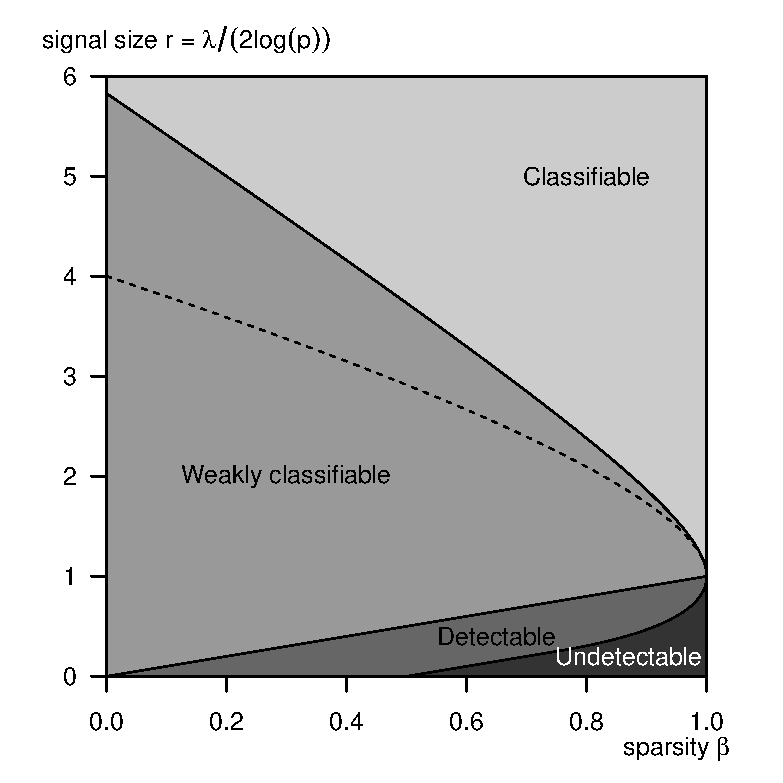
\includegraphics[width=0.55\textwidth]{./phase_diagram_chisquared.eps}
      % 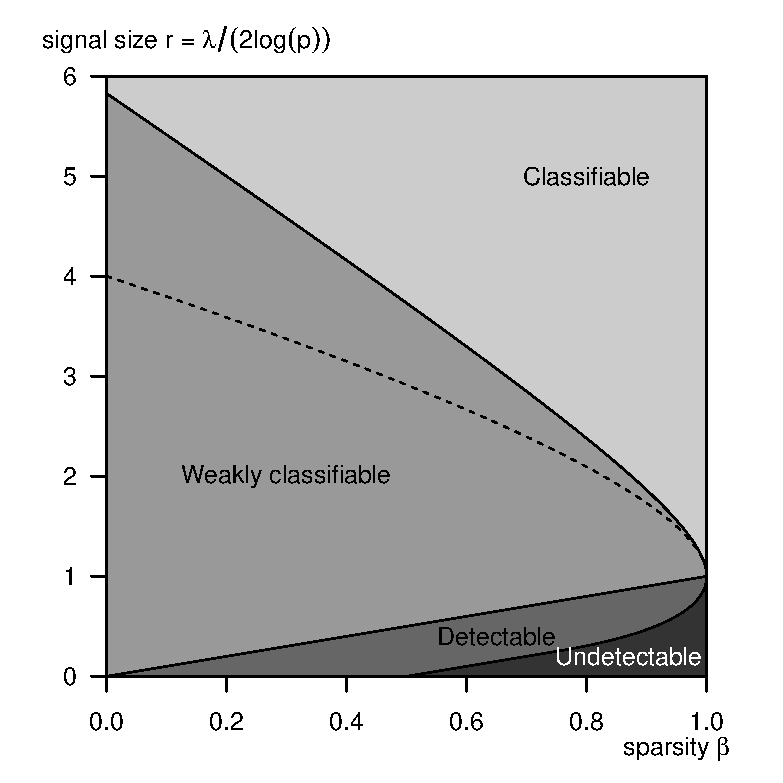
\includegraphics[width=0.35\textwidth]{./phase_diagram_chisquared.eps}
      \caption{The phase transitions of the exact and approximate support recovery problems, described in Theorems \ref{thm:chi-squred-strong-boundary} and \ref{thm:chi-squred-weak-boundary}, and of the signal detection problem, described in \citep{donoho2004higher}. 
      The risk of exact support recovery \eqref{eq:risk-exact} can be made to vanish above the strong classification boundary \eqref{eq:strong-classification-boundary-chisquared} in the \emph{classifiable} region; conversely, the risk has liminf at least one.
      Similarly, the risk of approximate support recovery \eqref{eq:risk-approximate} can be made to vanish above the weak classification boundary \eqref{eq:weak-classification-boundary-chisquared} in the \emph{weakly classifiable} region; conversely, the risk has liminf at least one.
      Both boundaries are unaffected by the degrees-of-freedom parameter in the model.} 
      \label{fig:phase-chi-squared}
\end{figure}

\begin{remark}
Remarkably, the degree-of-freedom parameter $\nu$ does not affect the boundary \eqref{eq:strong-classification-boundary-chisquared}.
In simulations, we find the approximation by the asymptotic boundary to be quite accurate even in moderate dimensions, and largely unaffected by the degrees of freedom.
See Figure \ref{fig:phase-simulated-chi-squared} for numerical illustrations.
\end{remark}

As alluded to in Section \ref{subsec:motivation-additive} in the introduction, Theorem \ref{thm:chi-squred-strong-boundary} also allows us to compare the difficulties of one-sided versus two-sided additives for additive models under Gaussian errors.

\begin{remark}
The exact support recovery problem under the Gaussian additive error model \eqref{eq:model-additive} was studied \cite{gao2018fundamental}.
where the same parametrization of sparsity \eqref{eq:signal-sparsity} was adopted. 
The signal sizes of the non-zero mean shifts in $\mu(i)$ were parametrized in a similiar fashion as \eqref{eq:signal-size} between $\sqrt{2\underline{r}\log{p}}$ and $\sqrt{2\overline{r}\log{p}}$;
it was assumed that $0<\underline{r}\le\overline{r}$, and only one-sided alternatives were considered.
Interestingly, under one-sided alternatives in the additive model, a phase transition in the $r$-$\beta$ plane also exists for the exact support recovery problem.
However, its boundary becomes
\begin{equation} \label{eq:strong-classification-boundary-additive}
    \widetilde{g}(\beta) = \left(1 + \sqrt{1-\beta}\right)^2,
\end{equation}
which is strictly less than the required signal sizes in the two-sided case in \eqref{eq:strong-classification-boundary-chisquared}, except in the extremely sparse case $\beta = 1$.
In particular, as the problem becomes denser ($\beta\to0$), the required signal size in the one-sided additive model \eqref{eq:strong-classification-boundary-additive} approaches $2$, while the required signal size in the chi-square (two-sided additive) model \eqref{eq:strong-classification-boundary-chisquared} approaches $3+2\sqrt{2} \approx 5.828$; almost a 3-fold increase.
\end{remark}


\subsection{FDR-controlling procedures}
\label{subsec:FDR-controlling-procedures}

Introduce the Benjamini-Hochberg procedure here.

\subsection{The weak classification boundary}
\label{subsec:weak-classification-boundary}

We now state our second main result, characterizing the phase-transition phenomenon in the approximate support recovery problem under the chi-square model.

\begin{theorem} \label{thm:chi-squred-weak-boundary}
Consider the high-dimensional chi-squared model \eqref{eq:model-chisq}.
Let the signal $\lambda$ be as described in Theorem \ref{thm:chi-squred-strong-boundary}.
The function 
\begin{equation} \label{eq:weak-classification-boundary-chisquared}
    h(\beta) = \beta
\end{equation}
characterizes the phase transition of approximate support recovery problem.
Specifically, if $\underline{r} > {h}(\beta)$, then the Benjamini-Hochberg procedure $\widehat{S}_p$ (defined in \eqref{eq:BH-procedure}) with FDR levels $\alpha=\alpha_p$ satisfying
\begin{equation} \label{eq:FDR-rate-to-zero}
    \alpha\to 0,\quad \text{and} \quad \alpha p^\delta\to\infty \text{  for any } \delta>0.
\end{equation}
achieves asymptotically approximate support recovery in the sense of \eqref{eq:approx-recovery-success}. 

Conversely, if $\overline{r} < {h}(\beta)$, then approximate support recovery asymptotically fails in the sense of \eqref{eq:approx-recovery-failure} for all thresholding procedures.
\end{theorem}

\begin{remark}
the detection boundary and weak classification boundary under one-sided alternatives are identical to that in the two-sided problems. (see Theorem \ref{thm:chi-squred-weak-boundary} below).
\end{remark}